%
% Packages
%
\documentclass[10pt]{article} 
\usepackage[landscape]{geometry}
\usepackage{url}
\usepackage{multicol}
\usepackage{amsmath}
\usepackage{esint}
\usepackage{bigints}
\usepackage{amsfonts}
\usepackage{xcolor}
\usepackage{tikz}
\usepackage{amsmath,amssymb}
\usepackage{colortbl}
\usepackage{xcolor}
\usepackage{mathtools}
\usepackage{amsmath,amssymb}
\usepackage{enumitem}
\usepackage{xhfill}
\usepackage[french]{babel}
\usepackage[utf8]{inputenc}
\usepackage{parskip}
\usepackage[T1]{fontenc}
\usepackage{mathrsfs}
\usepackage{pgfplots}
\usepackage{algorithm} % For writing pseudocode
\usepackage{algpseudocode} % For pseudocode layout
\usepackage{listings}
\usepackage{xcolor}


\usetikzlibrary{calc}
\usetikzlibrary{decorations.pathmorphing}
\usetikzlibrary{pgfplots.groupplots}
\pgfplotsset{compat=1.17}
\makeatletter

%
% Math
%
\newcommand{\Real}{\mathbb R}
\newcommand{\RPlus}{\Real^{+}}
\newcommand{\norm}[1]{\left\Vert#1\right\Vert}
\newcommand{\abs}[1]{\left\vert#1\right\vert}
\newcommand{\setn}[1]{\left\{#1\right\}_{\scriptscriptstyle n \ge 1}}
\newcommand{\set}[1]{\left\{#1\right\}}
\newcommand{\seq}[1]{\left<#1\right>}
\newcommand{\eps}{\varepsilon}
\newcommand{\To}{\longrightarrow}
\newcommand{\Prob}{\rm{P}}
\newcommand{\F}{\mathcal{F}}
\newcommand{\h}{\mathcal{H}}
\newcommand{\M}{\mathcal{M}}
\newcommand{\X}{\mathcal{X}}
\newcommand{\N}{\mathcal{N}}
\newcommand{\E}{{\rm E}}
\newcommand{\Hnull}{{\rm H}_{0}}
\newcommand{\Hone}{{\rm H}_{1}}
\newcommand{\Var}{{\rm Var}}
\newcommand{\Cov}{{\rm Cov}}
\newcommand{\sign}{{\rm sign}}
\newcommand{\med}{{\rm med}}
\newcommand{\tr}{{\rm tr}}
\newcommand{\T}{{\text{\tiny \rm T}}}
\newcommand{\minf}{- \, \infty}
\newcommand{\intervalle}[4]{\mathopen{#1}#2\mathpunct{},#3\mathclose{#4}}
\newcommand{\intervalleff}[2]{\intervalle{[}{#1}{#2}{]}}
\newcommand{\intervalleof}[2]{\intervalle{]}{#1}{#2}{]}}
\newcommand{\intervallefo}[2]{\intervalle{[}{#1}{#2}{[}}
\newcommand{\intervalleoo}[2]{\intervalle{]}{#1}{#2}{[}}
\newcommand*\conj[1]{\overline{#1}}
\newcommand*\mean[1]{\overline{#1}}

%
% Setup
%
\geometry{
  top=5mm,    % Minimal top margin
  %bottom=5mm, % Minimal bottom margin
  left=5mm,   % Minimal left margin
  right=5mm,   % Minimal right margin
  textheight=220mm
}
\title{Deep Learning Cheat Sheet}

% Paragraph and column formatting
\setlength{\parindent}{0pt}          % No indentation at the start of a paragraph
\setlength{\parskip}{1pt plus 1pt minus 0.5pt}  % Moderate space between paragraphs
\setlength{\columnsep}{10pt}         % Moderate space between columns

% Line and baseline spacing
\setlength{\baselineskip}{2pt}      % Adequate baseline skip
\linespread{0.4}                     % Reset line spacing to normal

% Space around displayed math
\setlength{\abovedisplayskip}{3pt}
\setlength{\belowdisplayskip}{3pt}
\setlength{\abovedisplayshortskip}{3pt}
\setlength{\belowdisplayshortskip}{3pt}

%
% Commands
%
\newcommand*\bigcdot{\mathpalette\bigcdot@{.5}}
\newcommand*\bigcdot@[2]{\mathbin{\vcenter{\hbox{\scalebox{#2}{$\m@th#1\bullet$}}}}}
\makeatother
\newcommand{\hr}{\centerline{\rule{3.5in}{1pt}}}
%\colorbox[HTML]{e4e4e4}{\makebox[\textwidth-2\fboxsep][l]{texto}
\newcommand{\nc}[2][]{%
\vspace{-.16cm}
\tikz \draw [draw=black, ultra thick, #1]
    ($(current page.center)-(0.5\linewidth,0)$) --
    ($(current page.center)+(0.5\linewidth,0)$)
    node [midway, fill=white] {#2};
}% tomado de https://tex.stackexchange.com/questions/179425/a-new-command-of-the-form-tex


%
% Styles
%
\tikzstyle{mybox} = [draw=black, fill=white, very thick,
rectangle, rounded corners, inner sep=2pt, inner ysep=7pt]
\tikzstyle{fancytitle} =[fill=black, text=white, font=\bfseries]

\newlength{\boxsize}
\setlength{\boxsize}{0.247\textwidth}
\raggedcolumns


%
% Listing
%

% Définition du style Monokai
\definecolor{codegreen}{rgb}{0,0.6,0}
\definecolor{codegray}{rgb}{0.5,0.5,0.5}
\definecolor{codepurple}{rgb}{0.58,0,0.82}
\definecolor{backcolour}{rgb}{0.95,0.95,0.92}
\lstdefinestyle{monokai}{
    %backgroundcolor=\color{backcolour},   
    commentstyle=\color{codegreen},
    keywordstyle=\color{magenta},
    numberstyle=\tiny\color{codegray},
    stringstyle=\color{codepurple},
    basicstyle=\ttfamily\footnotesize,
    breakatwhitespace=false,         
    breaklines=true,                 
    keepspaces=true,                 
    numbers=none,                    
    numbersep=5pt,                  
    showspaces=false,                
    showstringspaces=false,
    showtabs=false,                  
    tabsize=2,
    xleftmargin=0.01\textwidth,
    xrightmargin=0.00\textwidth,
}
\lstset{style=monokai}

%###############################################################################################
%
%                                         Document
%
%###############################################################################################



\begin{document}

%---------------------------------
% Title
%---------------------------------
\begin{center}
    {\huge{\textbf{Deep Learning Cheat Sheet}}}\\
\end{center}
\vspace{-0.1cm}

\begin{multicols*}{4}
    
    %---------------------------------
    % Perforamnce Measures
    %---------------------------------
    \begin{tikzpicture}
        \node [mybox] (box){%
            \begin{minipage}{0.247\textwidth}
                Accuracy = $\dfrac{TP + TN}{ TP + TN + FP + FN}$\\
                Error Rate = $1 - accuracy$\\
                Precision = $\dfrac{TP}{ TP + FP}$\\
                \begin{multicols*}{2}
                    TPR = $\dfrac{TP}{TP + FN}$\\
                    TNR = $\dfrac{TN}{TN + FP}$\\
                    FPR = $\dfrac{FP}{FP + TN}$\\
                    FNR = $\dfrac{FN}{FN + TP}$\\
                \end{multicols*}
                F1-score = $\dfrac{2\cdot Precision \cdot TPR}{ Precision + TPR}$\\
                Specificity = $\dfrac{TP}{TN + FP}$\\
                AUC = $\displaystyle\int_{0}^{1} TPR \cdot dFPR$\\
                Macro Average = $\dfrac{1}{n} \displaystyle\sum_{i=1}^{n} avg_i$\\
                Micro Average = $\dfrac{\displaystyle\sum_{i=1}^{n} TP_i}{\displaystyle\sum_{i=1}^{n} TP_i + \displaystyle\sum_{i=1}^{n} FP_i}$
            \end{minipage}
        };
        \node[fancytitle, right=10pt] at (box.north west) {Evaluation Metrics};
    \end{tikzpicture}
    %---------------------------------
    
    %---------------------------------
    % Bias & Variance
    %---------------------------------
    \begin{tikzpicture}
        \node [mybox] (box){%
            \begin{minipage}{0.247\textwidth}
                \textbf{Bias}$(h_\theta) = \mathbb{E}[h_\theta, D] - f$\\
                \textbf{Var}$(h_\theta) = \mathbb{E}[(h_\theta, D - \mathbb{E}[h_\theta, D])^2]$\\
                \textbf{MSE} = $\text{Bias}(h_\theta)^2 + \text{Var}(h_\theta) + \sigma^2$\\
                $$
                    \underbrace{\text{Underfitting}}_{\text{high bias, low variance}} \qquad \underbrace{\text{Overfitting}}_{\text{low bias, high variance}}
                $$
                
            \end{minipage}
        };
        \node[fancytitle, right=10pt] at (box.north west) {Bias \& Variance};
    \end{tikzpicture}
    %---------------------------------
    
    %---------------------------------
    % Data Preparation
    %---------------------------------
    \begin{tikzpicture}
        \node [mybox] (box){%
            \begin{minipage}{0.247\textwidth}
                \textbf{Min-max [0,1]}: $x' = \dfrac{\left(x-x_{min}\right)}{\left(x_{max}-x_{min}\right)}$\\
                \textbf{Min-max [-1,1]}: $x' = 2 \cdot min\_max(x) -1$ \\
                min-max doesn't handle outliers.\\
                \textbf{Z-norm}: $x' = \dfrac{\left(x-\mu\right)}{\sigma}$\\
                \textbf{Scaling \& Centering}\\
                Scaling improves the numerical stability, the convergence speed and accuracy of the learning algorithms. Centering improves the robustness of the learning algorithms
            \end{minipage}
        };
        \node[fancytitle, right=10pt] at (box.north west) {Data Preparation};
    \end{tikzpicture}
    %---------------------------------
    
    %---------------------------------
    % Activation Functions
    %---------------------------------
    \begin{tikzpicture}
        \node [mybox] (box){%
            \begin{minipage}{0.247\textwidth}
                \nc{Sigmoid} $\sigma(z) = \frac{1}{1 + e^{-z}}$ --- Smooth and differentiable. Used in output layers for binary classification.\\
                \nc{Hyperbolic Tangent (tanh)}
                $f(z) = \tanh(z)$ --- Smooth, differentiable, output centered around 0. Used in LSTM.\\
                
                \nc{Rectified Linear Unit (ReLU)}
                $f(z) = \max(0, z)$ --- Non-linear, used as a standard, but has dying units problem for $z<0$.\\
                
                \nc{Leaky ReLU}
                $f(z) = \begin{cases} z & \text{if } z \geq 0 \\ \alpha z & \text{if } z < 0 \end{cases}$ --- Addresses dying units problem with a small $\alpha$ (typical $\alpha = 0.01$).\\
                
                
                \nc{Exponential Linear Unit (ELU)}
                $f(z) = \begin{cases} z & \text{if } z \geq 0 \\ \alpha(e^z - 1) & \text{if } z < 0 \end{cases}$ --- Similar to Leaky ReLU but more computationally expensive.\\
                
                
                \nc{Softmax}
                $f(z_i) = \frac{e^{z_i}}{\sum_{j=0}^{K-1} e^{z_j}}$ --- Used in the last layer for multi-class classification, outputs a probability distribution.
            \end{minipage}
        };
        \node[fancytitle, right=10pt] at (box.north west) {Activation Functions};
    \end{tikzpicture}
    %---------------------------------
    
    %---------------------------------
    % Universal Approximation Theorem
    %---------------------------------
    
    \begin{tikzpicture}
        \node [mybox] (box){%
            \begin{minipage}{0.247\textwidth}
                A feedforward network with a linear output layer and at least one hidden layer with a non-linear activation function (e.g. sigmoid) can approximate a large class of functions 
                $f:\mathbb{R}^n \rightarrow \mathbb{R}^m$ with arbitrary accuracy, provided that the network is given enough hidden units.
            \end{minipage}
        };
        \node[fancytitle, right=10pt] at (box.north west) {Universal Approximation Theorem};
    \end{tikzpicture}
    %---------------------------------
    
    %---------------------------------
    % Curse of Dimensionality
    %---------------------------------
    \begin{tikzpicture}
        \node [mybox] (box){%
            \begin{minipage}{0.247\textwidth}
                when the dimensionality increases, the volume of the space increases so fast that the
                available data become sparse. This sparsity is problematic for any method that requires statistical significance. In order to obtain a statistically sound and reliable result, the amount of
                data needed to support the result often grows exponentially with the dimensionality
            \end{minipage}
        };
        \node[fancytitle, right=10pt] at (box.north west) {Curse of Dimensionality};
    \end{tikzpicture}
    %---------------------------------
    
    %---------------------------------
    % Gradient Descent
    %---------------------------------
    \begin{tikzpicture}
        \node [mybox] (box){%
            \begin{minipage}{0.247\textwidth}
                \begin{algorithmic}[1]
                    \State Initialize parameter vector $\theta_0$
                    \Repeat
                    \State Compute the gradient of the cost function at current position $\theta_t$: $\nabla_{\theta} J(\theta_t)$
                    \State Update the parameter vector by moving against the gradient:
                    $
                        \theta_{t+1} = \theta_t - \alpha \cdot \nabla_{\theta} J(\theta_t)
                    $
                    \State where $\alpha$ is the learning rate.
                    \Until{change in $\theta$ is small}
                \end{algorithmic}
                \nc{MSE}\\
                $$
                    J_{MSE}(\theta) = \frac{1}{2m} \sum_{i=1}^m (\hat{y}(i) - y(i))^2
                $$
                where:
                \begin{itemize}
                    \item \( \hat{y}(i) = h_{\theta}(x(i)) \) is the prediction of the model,
                    \item \( y(i) \) is the true outcome,
                    \item \( m \) is the number of training examples.
                \end{itemize}
                \begin{multline*}
                    \\\nabla_w J_{MSE}(w, b) =\\ \frac{1}{m} \sum_{i=1}^m \hat{y}(i) \cdot (1 - \hat{y}(i)) \cdot (\hat{y}(i) - y(i)) \cdot x(i)\\
                    \nabla_b J_{MSE}(w, b) = \\\frac{1}{m} \sum_{i=1}^m \hat{y}(i) \cdot (1 - \hat{y}(i)) \cdot (\hat{y}(i) - y(i))
                \end{multline*}
                
                \nc{Cross Entropy}
                \begin{multline*}J_{CE}(\theta) = - \sum_{i=1}^m y(i) \cdot \log h_\theta(x(i)) + \\(1 - y(i)) \cdot \log (1 - h_\theta(x(i))) \end{multline*}
                where:
                \begin{itemize}
                    \item \( p_\theta(y(i) \mid x(i)) \) is the probability model parameterized by \( \theta \), predicting the probability of the true class \( y(i) \) given the input \( x(i) \),
                    \item \( m \) is the number of observations or data points in the dataset.
                \end{itemize}
                $\nabla_w J_{CE}(w, b) = \frac{1}{m} \sum_{i=1}^m (\hat{y}(i) - y(i)) \cdot x(i)$
                
                $\nabla_b J_{CE}(w, b) = \frac{1}{m} \sum_{i=1}^m (\hat{y}(i) - y(i))$
            \end{minipage}
        };
        \node[fancytitle, right=10pt] at (box.north west) {Gradient Descent};
    \end{tikzpicture}
    %--------------------------------
    
    %---------------------------------
    % Gradient Descent Variants
    %---------------------------------
    \begin{tikzpicture}
        \node [mybox] (box){
            \begin{minipage}{0.247\textwidth}
                \nc{BGD}: Smooth, not wiggling, strictly decreasing cost, many epochs needed, choose larger learning rate, no out-of-core support - all data in RAM (~m), easy to parallelise.
                \nc{SGD}: Wiggling, needs smoothing, wiggles around minimum, not necessarily decreasing cost, few epochs needed, choose smaller learning rate, out-of-core support - not all data to be kept in RAM of a single machine, not easy to parallelise.
                \nc{MBGD}: Slightly wiggling, wiggles around minimum, typically decreasing cost, less epochs than BGD, more than SGD needed, choose medium learning rate (dependent on model), out-of-core support - not all data to be kept in RAM of a single machine, easy to parallelise.
            \end{minipage}
        };
        \node[fancytitle, right=10pt] at (box.north west) {Gradient Descent Variants};
    \end{tikzpicture}
    
    %---------------------------------
    % Compute Graph
    %---------------------------------
    \begin{tikzpicture}
        \node [mybox] (box){%
            \begin{minipage}{0.247\textwidth}
                \begin{tikzpicture}[node distance=1cm]
                    \node (input) at (0,0) {$a^{[l-1]}$};
                    \node (weights) at (1,1) {$\textbf{W}^{[l]}$};
                    \node (bias) at (1,-1) {$\textbf{b}^{[l]}$};
                    \node (layer) at (3,0) {$Layer\ l$};
                    \node (output) at (5,0) {$a^{[l]}$}; 
                    \draw[-latex] (input) -- (layer);
                    \draw[-latex] (weights) -- (layer);
                    \draw[-latex] (bias) -- (layer);
                    \draw[-latex] (layer) -- (output);
                \end{tikzpicture}
                \begin{align*}
                    \mathbf{W}^{[l]} & = \begin{pmatrix}
                                             w_{11}       & \cdots & w_{1n^{[l-1]}}        \\
                                             \vdots       & \ddots & \vdots                \\
                                             w_{n^{[l]}1} & \cdots & w_{n^{[l]}n^{[l-1]}}
                                         \end{pmatrix} \\
                    \mathbf{a}^{[l]} & = \begin{pmatrix}
                                             a_{1}  \\
                                             \vdots \\
                                             a_{n^{[l]}}
                                         \end{pmatrix}                                                                      \\
                    \mathbf{b}^{[l]} & = \begin{pmatrix}
                                             b_{1}  \\
                                             \vdots \\
                                             b_{n^{[l]}}
                                         \end{pmatrix}
                \end{align*}
                
                $\textbf{a}^{[l]} = \sigma^{[l]}(\textbf{z}^{[l]})    $                                                                            \\
                $\textbf{z}^{[l]} = \textbf{W}^{[l]} \cdot \textbf{a}^{[l-1]} + \textbf{b}^{[l]} \quad \text{with } \textbf{a}^{[0]} = \textbf{x}$
            \end{minipage}
        };
        \node[fancytitle, right=10pt] at (box.north west) {Compute Graph};
    \end{tikzpicture}
    %---------------------------------
    
    %---------------------------------
    % Backpropagation
    %---------------------------------
    \begin{tikzpicture}
        \node [mybox] (box){%
            \begin{minipage}{0.247\textwidth}
                \nc{Matrix Notation}
                \begin{align*}
                    \frac{\partial L}{\partial \textbf{z}^{[l]}}   & = \frac{\partial L}{\partial \textbf{a}^{[l]}} * \frac{d\sigma^{[l]}(\textbf{z}^{[l]})}{dz}                    \\
                    \frac{\partial L}{\partial \textbf{W}^{[l]}}   & = \frac{\partial L}{\partial \textbf{z}^{[l]}} \cdot \left(\textbf{a}^{[l-1]}\right)^T                         \\
                    \frac{\partial L}{\partial \textbf{b}^{[l]}}   & = \frac{\partial L}{\partial \textbf{z}^{[l]}}                                                                 \\
                    \frac{\partial L}{\partial \textbf{a}^{[l-1]}} & = \left(\textbf{W}^{[l]}                          \right)^T \cdot \frac{\partial L}{\partial \textbf{z}^{[l]}} \\
                    \frac{\partial L}{\partial \textbf{z}^{[l]}}   & = \hat{\textbf{y}} - \textbf{y}                                                                                \\
                \end{align*}
                \nc{Full Batch}
                \begin{align*}
                    \frac{\partial L}{\partial \textbf{Z}^{[l]}}   & = \frac{\partial L}{\partial \textbf{A}^{[l]}} * \frac{d\sigma^{[l]}(\textbf{Z}^{[l]})}{dz}                                \\
                    \frac{\partial L}{\partial \textbf{W}^{[l]}}   & = \frac{\partial L}{\partial \textbf{Z}^{[l]}} \cdot \left(\textbf{A}^{[l-1]}\right)^T                                     \\
                    \frac{\partial L}{\partial \textbf{b}^{[l]}}   & = \frac{1}{m}\cdot\frac{\partial L}{\partial \textbf{Z}^{[l]}}\cdot    \begin{pmatrix} \vdots \\ 1 \\ \vdots \end{pmatrix} \\
                    \frac{\partial L}{\partial \textbf{A}^{[l-1]}} & = \left(\textbf{W}^{[l]}                          \right)^T \cdot \frac{\partial L}{\partial \textbf{Z}^{[l]}}             \\
                    \frac{\partial L}{\partial \textbf{Z}^{[l]}}   & = \hat{\textbf{Y}} - \textbf{Y}                                                                                            \\
                \end{align*}
                \nc{Batch Normalization}
                \begin{align*}
                    \frac{\partial L}{\partial \gamma} & = \frac{1}{m}\cdot\sum_{i=1}^{m} \frac{\partial L}{\partial \hat{a}^{(i)}} \cdot \frac{\partial \hat{a}^{(i)}}{\partial \gamma} \\
                                                       & = \frac{1}{m}\cdot\sum_{i=1}^{m} \frac{\partial L}{\partial \hat{a}^{(i)}} \cdot \hat{a}^{(i)}                                  \\
                    \frac{\partial L}{\partial \beta}  & = \sum_{i=1}^{m} \frac{\partial L}{\partial \hat{a}^{(i)}} \cdot \frac{\partial \hat{a}^{(i)}}{\partial \beta}                  \\
                                                       & = \sum_{i=1}^{m} \frac{\partial L}{\partial \hat{a}^{(i)}}
                \end{align*}
            \end{minipage}
        };
        \node[fancytitle, right=10pt] at (box.north west) {Backpropagation};
    \end{tikzpicture}
    %---------------------------------
    
    %---------------------------------
    % Vanishing Exploding Gradient
    %---------------------------------
    \begin{tikzpicture}
        \node [mybox] (box){%
            \begin{minipage}{0.247\textwidth}
                \nc{Xavier \& Heu Initialization}\\
                Sets the initial weights of a layer to values drawn from a uniform distribution with a range that depends on the number of input and output units in the layer. Specifically, the range is set to $[-r, r]$, where $r = \sqrt{\frac{6}{n_{in} + n_{out}}}$, and $n_{in}$ is the number of input units and $n_{out}$ is the number of output units. This range was chosen because it ensures that the variance of the outputs of each layer remains constant, which helps to prevent the vanishing or exploding gradient problem.\\
                \nc{Batch Normalization}
                We calculate the average $\mu_r$ and standard deviation $\sigma_r$ over the $m$ column vectors $z_r$ of the mini-batch according to:
                \begin{align*}
                    \mu_r    & = \frac{1}{m} \sum_{i=1}^m z_r^{[l](i)}                     \\
                    \sigma_r & = \sqrt{\frac{1}{m} \sum_{i=1}^m (z_r^{[l](i)} - \mu_r)^2}
                \end{align*}
                Now, the actual normalization of the logit matrix is as follows:
                $$\hat{Z}_r^{[l]} = \frac{Z_r^{[l]} - \mu_r}{\sigma_r + \epsilon}$$
                Finally, two addition parameter vectors are introduced that rescale the logits according to :
                $$\tilde{Z}_r^{[l]} = \gamma^{[l]} \cdot \hat{Z}_r^{[l]} + \beta^{[l]}$$
                \nc{Non Saturating Activation Function}\\
                To alleviate the saturation of sigmoid and tanh, we can use the ReLU activation function. It still suffer from dying units problem (when the input is negative, the gradient is 0).\\
                \nc{Gradient Clipping}\\
                If gradients values exceed a certain threshold, they are "clipped" or rescaled to a smaller value. This prevents the gradients from becoming too large and helps to stabilize the training process.
            \end{minipage}
        };
        \node[fancytitle, right=10pt] at (box.north west) {Vanishing Exploding Gradient};
    \end{tikzpicture}
    %---------------------------------
    
    %---------------------------------
    % Optimizers
    %---------------------------------
    \begin{tikzpicture}
        \node [mybox] (box){%
            \begin{minipage}{0.24\textwidth}
                \nc{Momentum} Uses a running average of gradients to smooth the optimization path.
                    {\small
                        \begin{align*}
                            m_t      & \leftarrow \beta m_{t-1} + \alpha \nabla_{\theta} J(\theta) \\
                            \theta_t & \leftarrow \theta_{t-1} - m_t
                        \end{align*}
                        Nesterov variant:
                        \begin{align*}
                            m_t      & \leftarrow \beta m_{t-1} + \alpha \nabla_{\theta} J(\theta_{t-1} - \beta m_{t-1}) \\
                            \theta_t & \leftarrow \theta_{t-1} - m_t
                        \end{align*}
                    }
                \nc{AdaGrad} Scaling down the gradient vector along the steepest dimensions.
                    {\small
                        \begin{align*}
                            s_t      & \leftarrow s_{t-1} + \nabla_{\theta} J(\theta_{t-1}) \cdot \nabla_{\theta} J(\theta_{t-1})            \\
                            \theta_t & \leftarrow \theta_{t-1} - \frac{\alpha}{\sqrt{s_t} + \epsilon} \cdot \nabla_{\theta} J(\theta_{t-1})
                        \end{align*}
                    }
                \nc{RMS Prop} A variant of AdaGrad using an exponentially decaying average of squared gradients.
                    {\small
                        \begin{align*}
                            s_t      & \leftarrow \beta s_{t-1} + (1 - \beta) \nabla_{\theta} J(\theta_{t-1}) \cdot \nabla_{\theta} J(\theta_{t-1}) \\
                            \theta_t & \leftarrow \theta_{t-1} - \frac{\alpha}{\sqrt{s_t} + \epsilon} \cdot \nabla_{\theta} J(\theta_{t-1})
                        \end{align*}
                    }
                \nc{Adam} Combines momentum and RMSProp to adapt the learning rate for each parameter.
                    {\small
                        \begin{align*}
                            m_t       & \leftarrow \beta_1 m_{t-1} + (1 - \beta_1) \nabla_{\theta} J(\theta_{t-1})                                       \\
                            s_t       & \leftarrow \beta_2 s_{t-1} + (1 - \beta_2) \nabla_{\theta} J(\theta_{t-1}) \cdot \nabla_{\theta} J(\theta_{t-1}) \\
                            \hat{m}_t & \leftarrow \frac{m_t}{1 - \beta_1^t}                                                                             \\
                            \hat{s}_t & \leftarrow \frac{s_t}{1 - \beta_2^t}                                                                             \\
                            \theta_t  & \leftarrow \theta_{t-1} - \frac{\alpha}{\sqrt{\hat{s}_t} + \epsilon} \cdot \hat{m}_t
                        \end{align*}
                    }
                \nc{Scheduler} Strategies to adjust the learning rate during training:
                \textbf{Performance scheduling}\\
                \textbf{Exponential scheduling:} $\alpha(t) = \alpha_0 \cdot 10^{-t/T}$\\
                \textbf{Power scheduling:} $\alpha(t) = \alpha_0 \cdot \left(1 + \frac{t}{T}\right)^{-c}$, where $c$ is typically set to 1.
            \end{minipage}
        };
        \node[fancytitle, right=10pt] at (box.north west) {Optimizers};
    \end{tikzpicture}
    %---------------------------------
    
    %---------------------------------
    % Regularization
    %---------------------------------
    \begin{tikzpicture}
        \node [mybox] (box){%
            \begin{minipage}{0.247\textwidth}
                \nc{Weight Penalty}\\
                Modify the loss function to include a penalty to big weights:
                \[
                    J(\theta) = J_0(\theta) + \lambda \cdot \Omega(W)
                \]
                where \(\Omega(W)\) is the penalty term:
                \begin{itemize}[noitemsep]
                    \item \textbf{L1:} \(\Omega(W) = \|W\|_1 = \sum|W_{ji}|\)
                    \item \textbf{L2:} \(\Omega(W) = \frac{1}{2} \|W\|_2^2 = \frac{1}{2} \sum(W_{ji}^2)\)
                \end{itemize}
                
                \nc{Dropout}\\
                Randomly drop neurons during training:
                \begin{itemize}[noitemsep]
                    \item Each neuron has probability \(p\) of being dropped.
                    \item Typical \(p\): 50% for hidden, 20% for input neurons.
                    \item During testing, scale weights by \(1 - p\).
                \end{itemize}
                
                \nc{Early Stopping}\\
                Stop training when validation error increases:
                \begin{itemize}[noitemsep]
                    \item Track validation error during training.
                    \item Save model parameters when validation error improves.
                    \item Stop if no improvement for a set number of steps.
                \end{itemize}
            \end{minipage}
        };
        \node[fancytitle, right=10pt] at (box.north west) {Regularization};
    \end{tikzpicture}
    %---------------------------------
    
    
    %---------------------------------
    % Autoencoder
    %---------------------------------
    \begin{tikzpicture}
        \node [mybox] (box){%
            \begin{minipage}{0.247\textwidth}
                \textbf{1. Data Compression / Dimensionality Reduction}\\
                - Train on input data, transmit encoded values instead of original.\\
                - Related to PCA with linear activations.\\
                
                \textbf{2. Feature Extraction}\\
                - Train on unlabeled data, use encoder output as features for classifiers.\\
                
                \textbf{3. De-noising}\\
                - Train with noisy data to predict clean data, useful for feature robustness.\\
                
                \textbf{4. Image In-painting}\\
                - Restore lost information in images, active research field.\\
                
                \textbf{5. Pre-training for Supervised Learning}\\
                - Unsupervised pre-training, followed by supervised fine-tuning improves deep networks.\\
            \end{minipage}
        };
        \node[fancytitle, right=10pt] at (box.north west) {Autoencoder};
    \end{tikzpicture}
    %---------------------------------
    
    %---------------------------------
    % Convolutional Neural Networks
    %---------------------------------
    \begin{tikzpicture}
        \node [mybox] (box){%
            \begin{minipage}{0.247\textwidth}
                \nc{Features}
                colors, terrain texture, size, presence of straight lines, border\\
                1. Extracting localized low-level features\\
                2. Incrementally allowing the system to appropriately bind together features and their relationships\\
                3. Gradually building up overall spatial invariance\\
                \nc{Pooling layer}
                Maxpooling after a convolution layer eliminates non-maximal values: it is a form of non-linear down-sampling that reduces computation for upper layers and provides a "summary" of the statistics of features in lower layers.\\
                \nc{Convolution layer}
                Different kernel sizes (3x3, 5x5, 7x7, etc.) allow the identification of features at different scales. Multiple layers of 3x3 kernels can implement other kernel sizes.\\
                The CONV layer’s parameters consist of a set of learnable filters. Every filter is small spatially (along width and height) but extends through the full depth of the input volume.\\
                We can compute the spatial size of the output volume as a function of the input volume size ($W$), the receptive field size of the Conv Layer neurons ($F$), the stride with which they are applied ($S$), and the amount of zero padding used ($P$) on the border.\\
                \nc{Input Volume}
                \textbf{Size}: $W_1 \times H_1 \times D_1$\\
                
                \nc{Hyperparameters}
                \textbf{K}: Number of conv filters\\
                \textbf{F}: Filter size (spatial extent)\\
                \textbf{S}: Stride\\
                \textbf{P}: The amount of zero padding\\
                
                \nc{Output Volume}
                \textbf{W2}: $\left\lfloor \frac{W_1 - F + 2P}{S} \right\rfloor + 1$\\
                \textbf{H2}: $\left\lfloor \frac{H_1 - F + 2P}{S} \right\rfloor + 1$\\
                \textbf{Size}: $W_2 \times H_2 \times K$\\
                
                \nc{Parameters}
                It introduces $\left(F \times F \times D_1\right) \times K$ weights plus $K$ biases.
            \end{minipage}
        };
        \node[fancytitle, right=10pt] at (box.north west) {Convolutional Neural Networks};
    \end{tikzpicture}
    %---------------------------------
    
    
    %---------------------------------
    % DeepCNN
    %---------------------------------
    \begin{tikzpicture}
        \node [mybox] (box){%
            \begin{minipage}{0.247\textwidth}
                \nc{LeNet5}\\
                - Premier CNN utilisé avec succès pour la reconnaissance des chiffres manuscrits (MNIST).\\
                - Utilisation de couches de convolution suivies de couches de sous-échantillonnage (pooling).\\
                \nc{AlexNet}\\
                - Introduction des CNN profonds avec huit couches apprises.\\
                - Utilisation de ReLU \\
                - Utilisation de Dropout\\
                - Utilisation de Data Augmentation\\
                \nc{VGGnet}\\
                - Profondeur accrue avec 16 à 19 couches.\\
                - Introduction de l'utilisation de petits filtres 3x3 dans toutes les couches de convolution.\\
                \nc{GoogleNet}\\
                - Introduction des Inceptions Modules: plusieurs tailles de filtres dans chaque couche.\\
                - Réduction des paramètres grâce à des couches 1x1 convolutions (depth projection)\\
                - injection of gradient at early stages
                \nc{ResNet}\\
                - Introduction des residual connections pour assurer la rétropropagation du gradient (gradient highway)\\
                - Résolution du problème de gradient vanishing dans les réseaux très profonds.\\
                - Batch Normalization\\
                - Xavier He Initialization\\
                - Bottleneck layers 1x1x64\\
                \nc{Pattern}\\
                - [Ajouter ici une brève description de l'innovation ou du concept clé lié au réseau "Pattern"].\\
            \end{minipage}
        };
        \node[fancytitle, right=10pt] at (box.north west) {DeepCNN};
    \end{tikzpicture}
    %---------------------------------
    
    %---------------------------------
    % Data Augmentation
    %---------------------------------
    \begin{tikzpicture}
        \node [mybox] (box){%
            \begin{minipage}{0.247\textwidth}
                \textbf{Strategies}\\
                pre-Augmentation, online augmentation\\
                \textbf{Methods}\\
                shear, zoom, color, rotation, flip, translation
            \end{minipage}
        };
        \node[fancytitle, right=10pt] at (box.north west) {Data Augmentation};
    \end{tikzpicture}
    %---------------------------------
    
    %---------------------------------
    % Transfer Learning
    %---------------------------------
    \begin{tikzpicture}
        \node [mybox] (box){%
            \begin{minipage}{0.247\textwidth}
                \textbf{Principle}\\
                using knowledge learned
                from tasks for which a lot of labelled data is available in
                settings where only little labelled data is available.
                \textbf{Keras Code}\\
                \textbf{MobileNet}\\
                \textbf{Strategies}\\
            \end{minipage}
        };
        \node[fancytitle, right=10pt] at (box.north west) {Transfer Learning};
    \end{tikzpicture}
    %---------------------------------
    
    %---------------------------------
    % Keras CNN
    %---------------------------------
    \begin{tikzpicture}
        \node [mybox] (box){%
            \begin{minipage}{0.247\textwidth}
                \nc{Model}
                \vspace{-0.5cm}
                \begin{lstlisting}[language=Python]
def build_model():
    visible = Input(shape=(32, 32, 3))
    # first feature extractor
    conv1 = Conv2D(32, kernel_size=3, activation='relu')(visible)
    drop1 = Dropout(0.2)(conv1)
    pool1 = MaxPooling2D(pool_size=(2, 2))(drop1)
    flat1 = Flatten()(pool1)
    # second feature extractor
    conv2 = Conv2D(32, kernel_size=6, activation='relu')(visible)
    drop2 = Dropout(0.2)(conv2)
    pool2 = MaxPooling2D(pool_size=(2, 2))(drop2)
    flat2 = Flatten()(pool2)
    # merge feature extractors
    merge = concatenate([flat1, flat2])
    # interpretation layer
    hidden1 = Dense(100, activation='relu')(merge)
    # prediction output
    output = Dense(n_classes, activation='softmax')(hidden1)
    model = Model(inputs=visible, outputs=output, name='exp2_functional')
    return model

clf = build_model()
clf.compile(loss='categorical_crossentropy', optimizer='adam', metrics=['accuracy'])
                \end{lstlisting}
                \nc{Data Augmentation}
                \vspace{-0.5cm}
                \begin{lstlisting}[language=Python]
datagen = ImageDataGenerator(
        rotation_range=20,
        width_shift_range=0.2,
        height_shift_range=0.2,
        horizontal_flip=True,
        shear_range=0.2,        
        zoom_range=0.2,        
        fill_mode='nearest')  
    
train_generator = datagen.flow(X_train, Y_train, batch_size=128)
test_generator = datagen.flow(X_test, Y_test, batch_size=128)

checkpoint_filepath = clf.name + '.keras'
                \end{lstlisting}
                \nc{Training}
                \vspace{-0.5cm}
                \begin{lstlisting}[language=Python]
history = clf.fit(
    train_generator,
    steps_per_epoch=100,
    epochs=15,
    validation_data=test_generator,
    validation_steps=10,
    callbacks=[ModelCheckpoint(checkpoint_filepath, save_best_only=True)]
)
                \end{lstlisting}
            \end{minipage}
        };
        \node[fancytitle, right=10pt] at (box.north west) {Keras CNN};
    \end{tikzpicture}
    %---------------------------------
    
    %---------------------------------
    % LSTM
    %---------------------------------
    \begin{tikzpicture}
        \node [mybox] (box){%
            \begin{minipage}{0.247\textwidth}
                \begin{center}
                    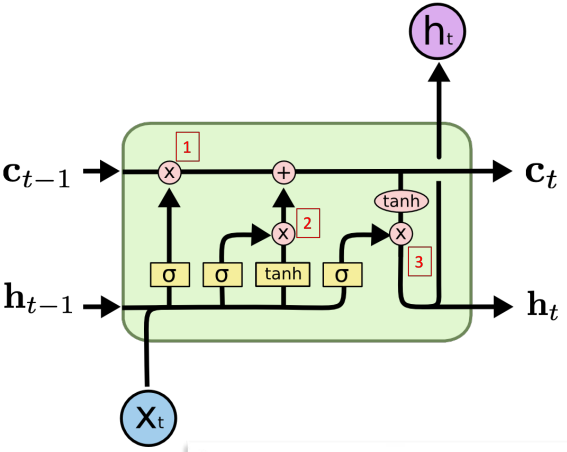
\includegraphics[width=\textwidth]{images/lstm_cell.png}
                \end{center}
                
                \textbf{Key Components}:
                \begin{itemize}[noitemsep]
                    \item (1) Forget Gate
                    \item (2) Input Gate
                    \item (3) output State
                    \item Cell state for storing long-term information.
                    \item Hidden state for short-term information.
                \end{itemize}
                
                \nc{Functioning}:
                \begin{center}
                    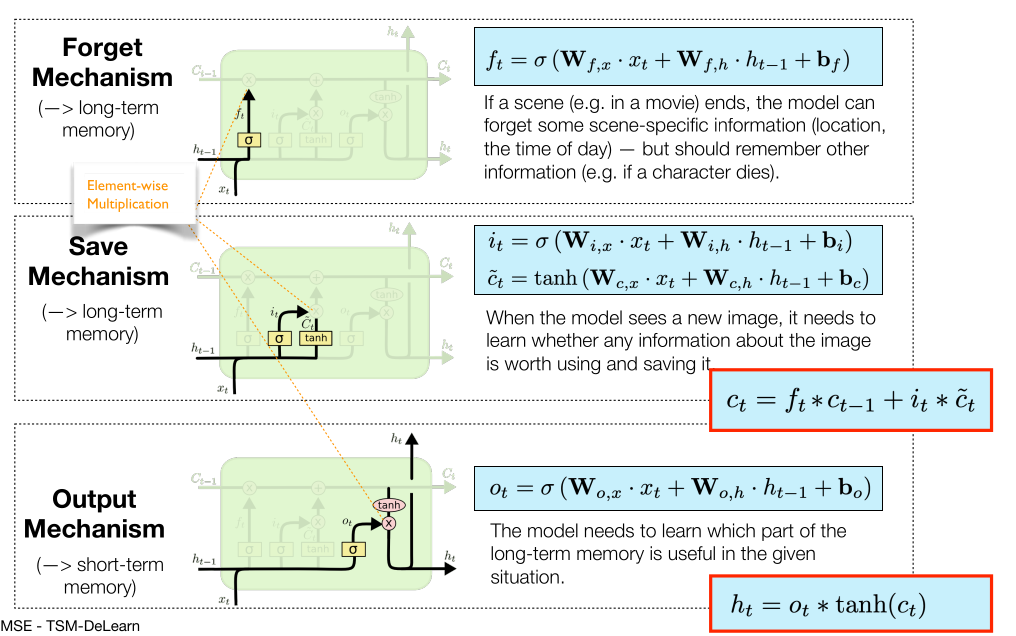
\includegraphics[width=\textwidth]{images/lstm_compute_graph.png}
                \end{center}
                Super-Highway for Backprop\\
                (+) Better at capturing long-range dependencies than standard RNNs, More effective in learning from large sequences of data.\\
                (-) More complex and computationally intensive to train than standard RNNs, May require more data to train effectively.\\
                \nc{Number of Weights}
                $4 x (N_{inputs} + N_{LSTMblocks} + bias) x N_{LSTMblocks}$\\
                Weights for 32 LSTM units and 2-dim inputs: 4 x (2 + 32 + 1) x 32 = 4480
                \nc{Vanishing Gradient}
                Vanishing/Exploding Gradients problem and the usual remedies in the
                context of RNNs (parameter initialisation, batchnorm, grad clipping)
            \end{minipage}
        };
        \node[fancytitle, right=10pt] at (box.north west) {LSTM};
    \end{tikzpicture}
    %---------------------------------
    
    %---------------------------------
    % RNN
    %---------------------------------
    \begin{tikzpicture}
        \node [mybox] (box){%
            \begin{minipage}{0.247\textwidth}
                \nc{Use Cases}
                \vspace{-0.2cm}
                
                - Sentiment Classification\\
                - Speech Recognition\\
                - Machine Translation\\
                - Captioning/Subtitling\\
                - Named Entity Recognition (NER)\\
                - Time Series Modelling, Prediction\\
                - Chatbots\\
                - Question/Answering\\
                - Sequence Generation\\
                
                \nc{Model Categories}
                \textbf{One-to-Many}\\
                - Image Captioning: Image -> Sequence of Words\\
                
                \textbf{Many-to-One}\\
                - Sentiment Classification: Sequence of Words -> Sentiment\\
                
                \textbf{Many-to-Many (1:1)}\\
                - Named Entity Recognition: Sequence of Words -> Sequence of Entity Classes\\
                
                \textbf{Many-to-Many (n:m)}\\
                - Machine Translation: Sequence of Words -> Sequence of Words\\
                - Speech Recognition: Sequence of Audio -> Sequence of Words\\
                - Chatbots: Sequence of Words -> Sequence of Words\\
                
                \textbf{Recurrent Cells}\\
                
                $\textbf{h}_t = f(\textbf{h}_{t-1}, \textbf{x}_{t})$\\
                $\textbf{z}_t = \textbf{W}_x \textbf{x}_t + \textbf{W}_h \textbf{h}_{t-1} + \textbf{b}_h$\\
                
                
                
                \textbf{Many-to-Many Example}\\
                \begin{center}
                    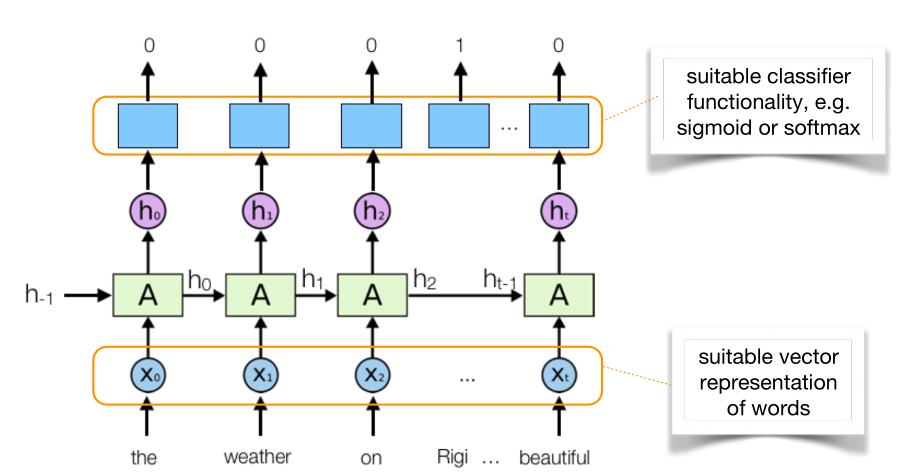
\includegraphics[width=0.9\textwidth]{images/rnn_many2many.png}
                \end{center}
                
                - Name classification with sequence lengths of up to ~18 characters works well with SimpleRNN.\\
                - Activity recognition with sequence lengths of up to ~128 steps has not worked well with SimpleRNN. Probably too long!\\
            \end{minipage}
        };
        \node[fancytitle, right=10pt] at (box.north west) {RNN};
    \end{tikzpicture}
    %---------------------------------
    
    %---------------------------------
    % RNN Keras
    %---------------------------------
    \begin{tikzpicture}
        \node [mybox] (box){%
            \begin{minipage}{0.247\textwidth}
                \nc{Name Classification}\\
                \vspace{-0.5cm}
                \begin{lstlisting}[language=Python]
# Model with multiple layers
model_multi_rnn = Sequential()
model_multi_rnn.add(SimpleRNN(units=64, input_shape=(maxlen, len_alphabet), return_sequences=True))
model_multi_rnn.add(SimpleRNN(units=32, return_sequences=False))
model_multi_rnn.add(Dense(len(languages), activation='softmax'))

model_multi_rnn.compile(loss='categorical_crossentropy', optimizer='adam', metrics=['accuracy'])
model_multi_rnn.summary()

# Train the model
log_multi_rnn = model_multi_rnn.fit(
    x=X_train,
    y=Y_train,
    batch_size=batch_size,
    epochs=nepochs,
    validation_data=(X_test, Y_test)
)
                \end{lstlisting}
                
                \nc{Activity Recognition (TS Classification)}\\
                \vspace{-0.5cm}
                \begin{lstlisting}[language=Python]
def build_RNN(input_shape, num_classes):
    model = Sequential()
    model.add(InputLayer(shape=input_shape))
    model.add(SimpleRNN(units=64, return_sequences=True))
    model.add(SimpleRNN(units=32))
    model.add(Dense(num_classes, activation='softmax'))
    model.compile(optimizer='adam', loss='categorical_crossentropy', metrics=['accuracy'])
    return model

model = build_RNN(input_shape=(128, 9), num_classes=6)
model.fit(X_train, y_train, batch_size=128, epochs=50)
            \end{lstlisting}
            \end{minipage}
        };
        \node[fancytitle, right=10pt] at (box.north west) {RNN Keras};
    \end{tikzpicture}
    %---------------------------------
    
    %---------------------------------
    % Word Embedding
    %---------------------------------
    \begin{tikzpicture}
        \node [mybox] (box){%
            \begin{minipage}{0.247\textwidth}
                \textbf{Word}\\
                Mapping of vocabulary of
                words into a n-dim
                vector space; n << v
                where v the size of the
                vocabulary.\\
                Encodes meaning of
                words so that words
                close in vector space are
                expected to have similar
                meanings
            \end{minipage}
        };
        \node[fancytitle, right=10pt] at (box.north west) {Word Embedding};
    \end{tikzpicture}
    %---------------------------------
    
    
    %---------------------------------
    % Sentiment Classification
    %---------------------------------
    \begin{tikzpicture}
        \node [mybox] (box){%
            \begin{minipage}{0.247\textwidth}
                \textbf{Data preparation}\\
                Remove html tags
                Replace punctuation
                with a space
                Remove single
                characters
                Remove multiple
                spaces\\
                \textbf{Splitting}\\
                Shuffle and apply
                split ratio\\
                \textbf{Tokenization}\\
                Mapping the words
                to integers by using
                a vocabulary of the
                most frequent
                words. Words not in
                most frequent
                words are skipped.
                Select parameter to
                specify 'most
                frequent words'\\
                \textbf{Cut and Pad}\\
                Cut and pad to
                fixed length.
                Select parameter
                with the sequence
                length.\\
            \end{minipage}
        };
        \node[fancytitle, right=10pt] at (box.north west) {Sentiment Classification};
    \end{tikzpicture}
    %---------------------------------
    
    
    %---------------------------------
    % GenRNN
    %---------------------------------
    \begin{tikzpicture}
        \node [mybox] (box){%
            \begin{minipage}{0.247\textwidth}
                System able to generate new consistent data from a seed. By consistent, we mean
                respecting temporal or spatial “structures” that have been
                learned from the input space.
                \textbf{Many to One}\\
                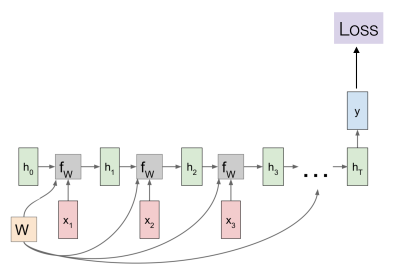
\includegraphics[width=\textwidth]{images/many2one.png}
                \textbf{Many to Many}\\
                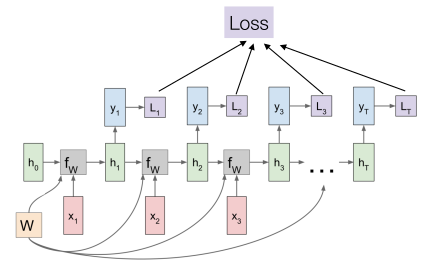
\includegraphics[width=\textwidth]{images/many2many.png}
            \end{minipage}
        };
        \node[fancytitle, right=10pt] at (box.north west) {GenRNN};
    \end{tikzpicture}
    %---------------------------------
    
    %---------------------------------
    % Attention
    %---------------------------------
    \begin{tikzpicture}
        \node [mybox] (box){%
            \begin{minipage}{0.247\textwidth}
                \textbf{Sequence to Sequence}\\
                A Seq2Seq model is learning to map sequences of
                different length in situations where the entire input
                sequence is required in order to start predicting the
                target sequence.
                \textbf{Attention}\\
                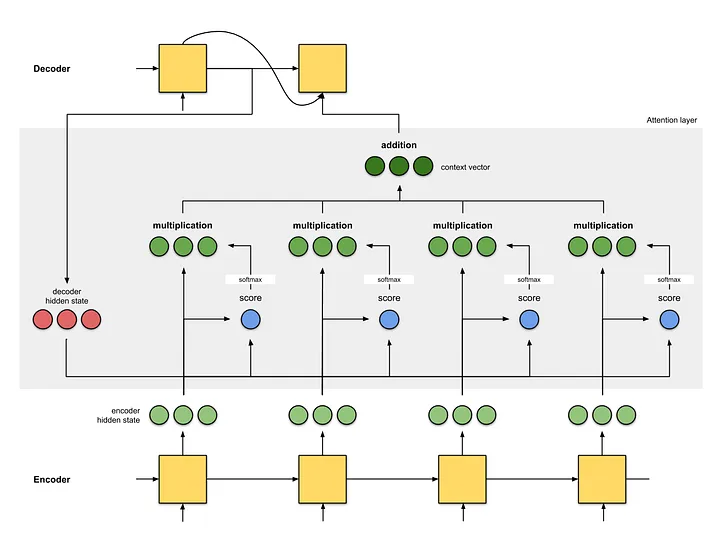
\includegraphics[width=\textwidth]{images/attention.png}
            \end{minipage}
        };
        \node[fancytitle, right=10pt] at (box.north west) {Attention};
    \end{tikzpicture}
    %---------------------------------
    
    %---------------------------------
    % Transformer
    %---------------------------------
    \begin{tikzpicture}
        \node [mybox] (box){%
            \begin{minipage}{0.247\textwidth}
                \textbf{High-Level Architecture}\\
                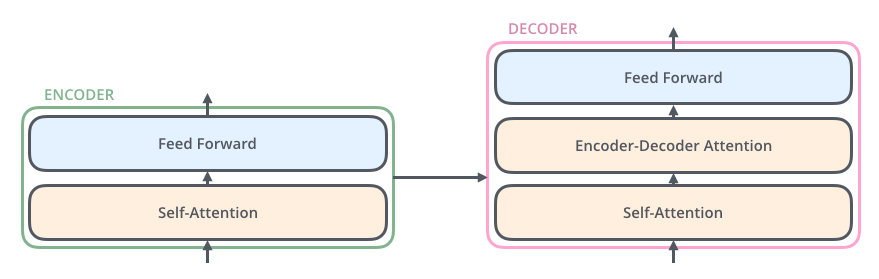
\includegraphics[width=\textwidth]{images/transformer.png}
                \textbf{Self-Attention}\\
                A self attention layer implements an attention
                mechanism by looking at adjacent inputs to provide an
                enhanced representation of a current input.
                $$ \text{Attention}(Q, K, V) = \text{softmax}\left(\frac{QK^T}{\sqrt{d_k}}\right)V $$
                \textbf{Full Architecture}\\
                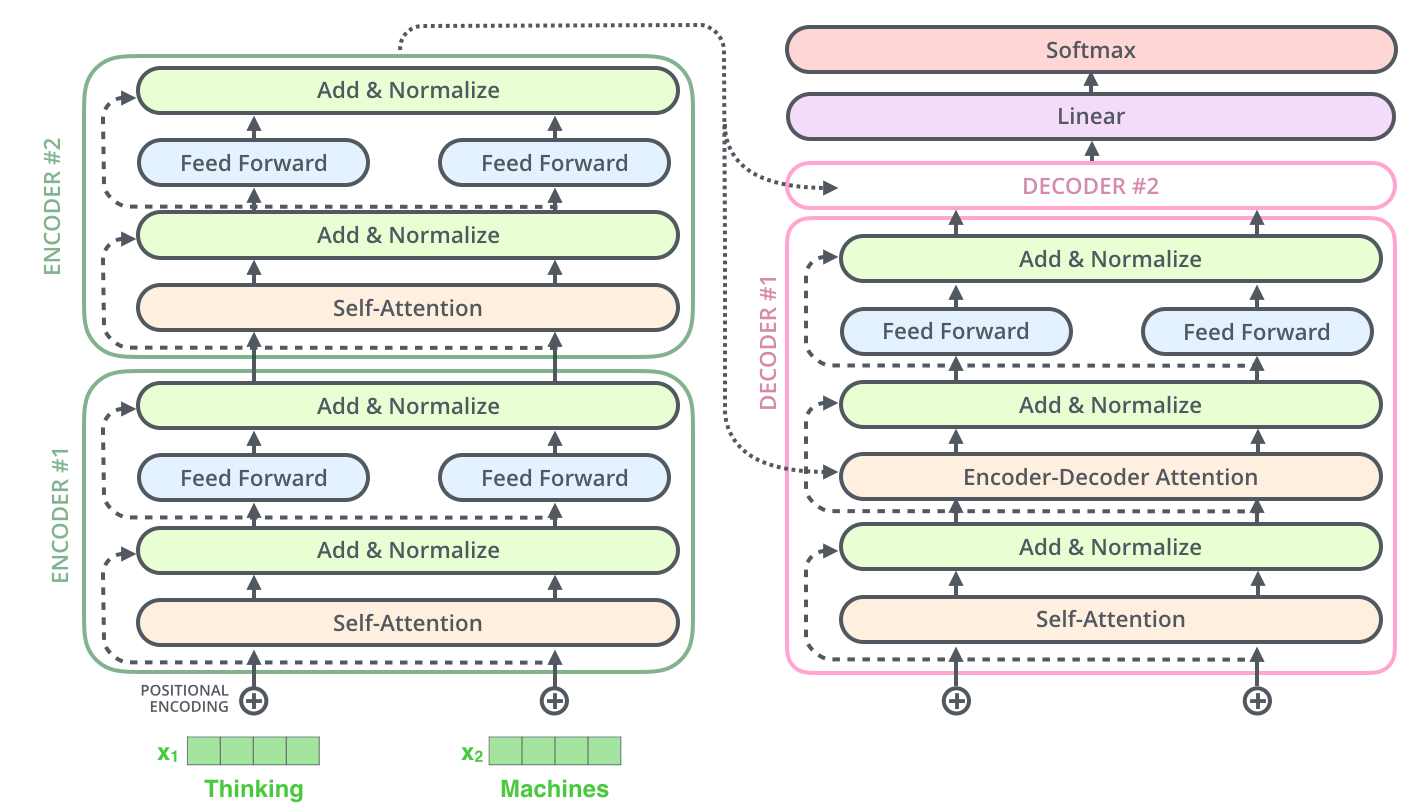
\includegraphics[width=\textwidth]{images/transformer_full.png}
            \end{minipage}
        };
        \node[fancytitle, right=10pt] at (box.north west) {Transformer};
    \end{tikzpicture}
    %---------------------------------
    
    %---------------------------------
    % Bayes
    %---------------------------------
    \begin{tikzpicture}
        \node [mybox] (box){%
            \begin{minipage}{0.247\textwidth}
                $$ P(C_k|x) = \frac{P(x|C_k) \cdot P(C_k)}{P(x)} $$                où
                \begin{itemize}[noitemsep]
                    \item $C_k$: Classe ciblée
                    \item $x$: Évidence
                    \item $P(C_k)$: Probabilité a priori de la classe $C_k$
                    \item $P(x|C_k)$: probability of observing x given class j
                    \item $P(C_k|x)$: Probabilité a posteriori de la classe $C_k$ après observation de $x$
                    \item $P(x)$: Probabilité de l'évidence $x$
                \end{itemize}
                avec 
                $$ P(x) = \sum_{\text{toutes classes } C_k} P(x|C_k) \cdot P(C_k) $$
                
                \nc{Classifier H/F:}
                \begin{itemize}
                    \item $P(C_f) = \frac{4}{70}, P(C_g) = \frac{66}{70}$
                    \item $p(x|C_g) = 0.8, p(x|C_f) = 0.2$
                    \item Calcul de $p(x)$:
                          $$ p(x) = 0.2 \times \frac{4}{70} + 0.8 \times \frac{66}{70} $$
                    \item Calcul de $P(C_f|x)$ et $P(C_g|x)$:
                          $ P(C_f|x) = \frac{0.2 \times \frac{4}{70}}{p(x)}, \quad P(C_g|x) = \frac{0.8 \times \frac{66}{70}}{p(x)} $
                \end{itemize}
                
                (+)Can deal with imbalanced dataset, prior can be changed
            \end{minipage}
        };
        \node[fancytitle, right=10pt] at (box.north west) {Bayes};
    \end{tikzpicture}
    %---------------------------------
    
\end{multicols*}

\end{document}

